\section{Related Work}

\begin{frame}{Related Work}
       \tableofcontents[sectionstyle=show/hide, hideothersubsections]
    \begin{center}
    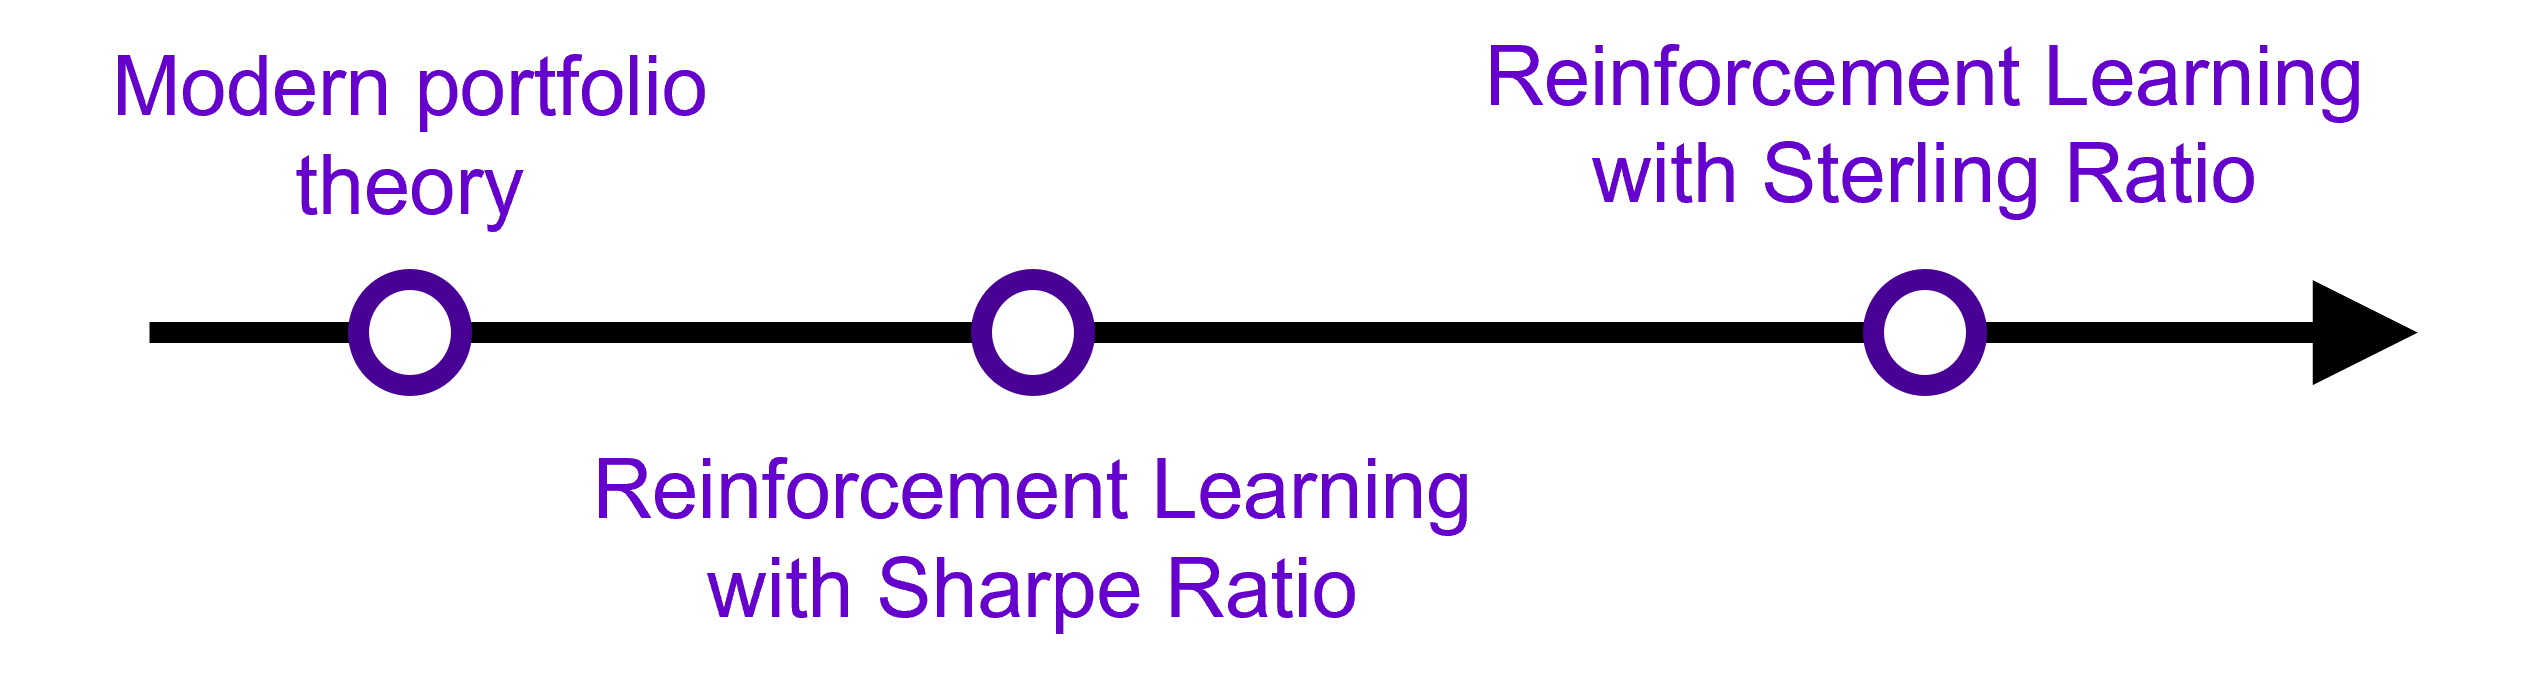
\includegraphics[width=10cm]{images/related.png}
    \end{center}
\end{frame}

\subsection{Modern Portfolio Theory}
\begin{frame}
\frametitle{Modern Portfolio Theory (MPT)}
\begin{columns}
\begin{column}{0.55\textwidth}
\begin{itemize}
    \item Use investment historical data to determine efficient frontier
    \item Can produce portfolio from given risk (variance)
    \item \alert{Does not incorporate alternative data}

\end{itemize}
\end{column}
\begin{column}{0.45\textwidth}
\begin{center}
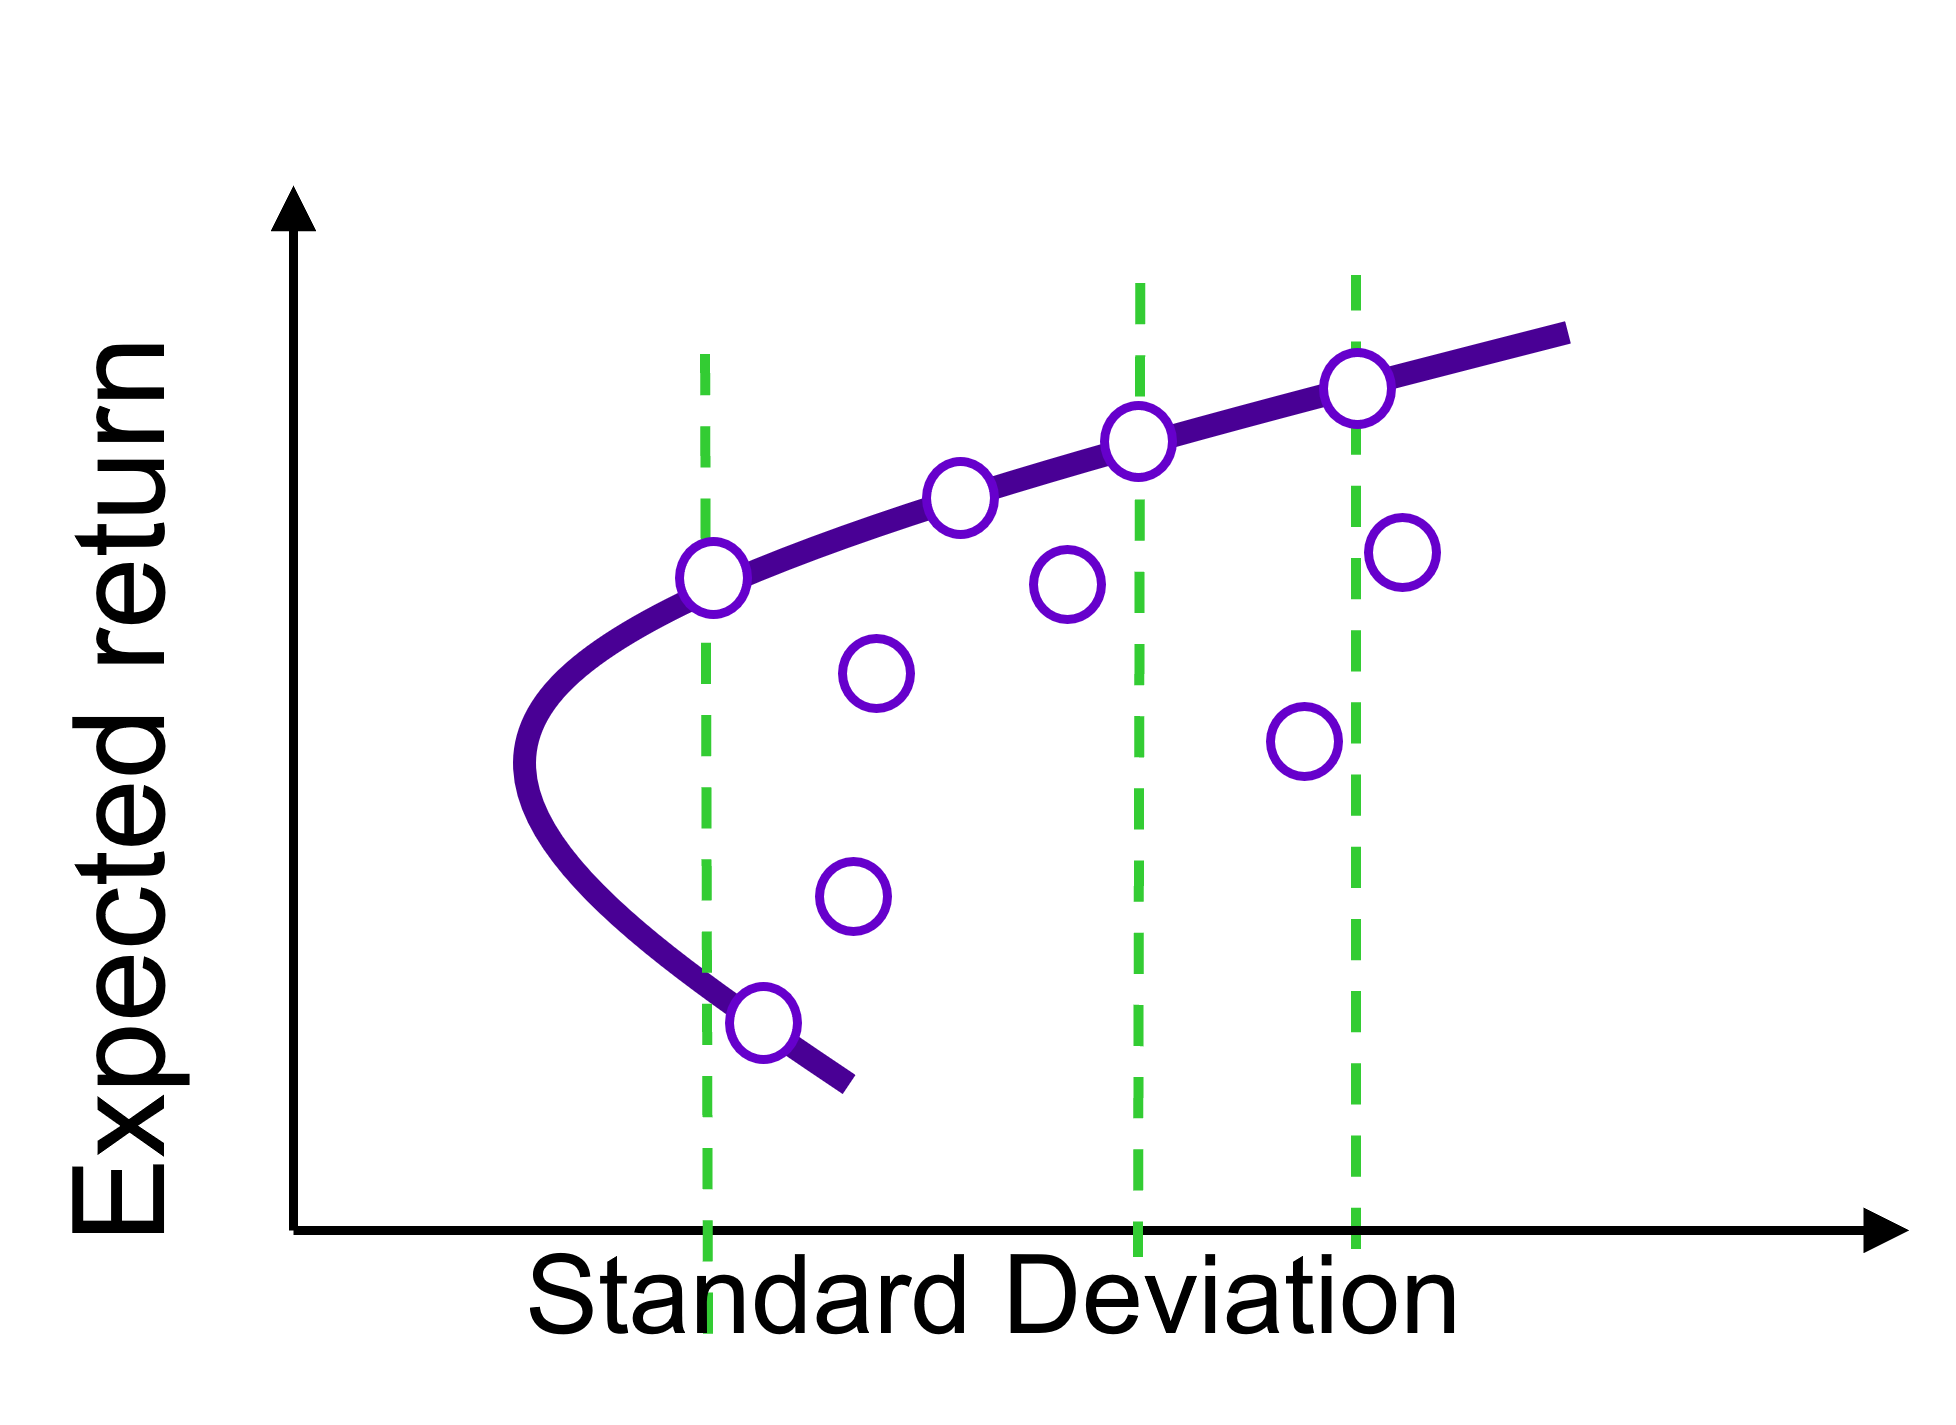
\includegraphics[width=4.8cm]{images/mpt_risk.png}
\end{center}
\end{column}
\end{columns}
\end{frame}


\subsection{Reinforcement Learning with Sharpe Ratio}
\begin{frame}{Reinforcement Learning with Sharpe Ratio}
John Moody's trading system used reinforcement learning to construct the optimal portfolio and used Sharpe Ratio as objective function.

\begin{block}{Sharpe Ratio}
\[ SR = \frac{E(R_a - R_b)}{\sigma_a}\]
\(R_a\): the return of the assert
\\
\(R_b\): the risk-free return
\\
\(E(R_a - R_b)\): the expected excess return of the assert
\\
\(\sigma_a\): standard deviation of the excess return.
\end{block}
\end{frame}



\subsection{Reinforcement Learning with Sterling Ratio}
\begin{frame}{Reinforcement Learning with Sterling Ratio}
\begin{block}{Problem}
Sharpe ratio is criticized for adjustment done based on variance rather than downside risk, \alert {penalty upon large positive returns}.
\end{block}
\begin{block}{Solution}
Use Sterling Ratio as objective function.
\[
Sterling Ratio=\frac{Annualized Average Return}{Maximum Drawdown}
\]
\end{block}

\end{frame}

\begin{frame}{Alternatives to Maximum Drawdown and  Sterling Ratio}
Maximum Drawdown is cumbersome to minimize.
Moody used DD to replace , the square root of the average of the
square of the negative returns, defined as
\[
DD_T = \sqrt{\cfrac{1}{T}\sum_{t=0}^{T}{min\{R_T,0\}^2}}
\]
And replace Sterling Ratio with downside deviation ratio (DDR)
\[
DDR_T = \frac{Average(R_T)}{DD_T}
\]
\end{frame}




\subsection{Comparison}
\begin{frame}{Comparison}
    \begin{columns}
    \begin{column}{0.5\textwidth}
    \begin{block}{DQN}
    
    \end{block}
    \begin{block}{TRPO/PPO}
    
    \end{block}
    \end{column}
    \begin{column}{0.5\textwidth}
        \begin{block}{DDPG/TD3}
    
    \end{block}
    \begin{block}{SAC}
    
    \end{block}
    \end{column}
    \end{columns}

\end{frame}